%%%%%%%%%%%%%%%%%%%%%%%%%%%%%%%%%%%%%%%%%
% FRI Data Science_report LaTeX Template
% Version 1.0 (28/1/2020)
% 
% Jure Demšar (jure.demsar@fri.uni-lj.si)
%
% Based on MicromouseSymp article template by:
% Mathias Legrand (legrand.mathias@gmail.com) 
% With extensive modifications by:
% Antonio Valente (antonio.luis.valente@gmail.com)
%
% License:
% CC BY-NC-SA 3.0 (http://creativecommons.org/licenses/by-nc-sa/3.0/)
%
%%%%%%%%%%%%%%%%%%%%%%%%%%%%%%%%%%%%%%%%%


%----------------------------------------------------------------------------------------
%	PACKAGES AND OTHER DOCUMENT CONFIGURATIONS
%----------------------------------------------------------------------------------------
\documentclass[fleqn,moreauthors,10pt]{ds_report}
\usepackage[english]{babel}

\graphicspath{{fig/}}




%----------------------------------------------------------------------------------------
%	ARTICLE INFORMATION
%----------------------------------------------------------------------------------------

% Header
\JournalInfo{FRI Natural language processing course 2022}

% Interim or final report
\Archive{Project report} 
%\Archive{Final report} 

% Article title
\PaperTitle{Cross lingual question answering} 

% Authors (student competitors) and their info
\Authors{Martin Božič, Matic Šincek, and Jakob Maležič}

% Advisors
\affiliation{\textit{Advisors: Slavko Žitnik}}

% Keywords
\Keywords{question-answering, cross-lingual, natural-language-processing}
\newcommand{\keywordname}{Keywords}
\newcommand{\verbatimfont}[1]{\renewcommand{\verbatim@font}{\ttfamily#1}}


%----------------------------------------------------------------------------------------
%	ABSTRACT
%----------------------------------------------------------------------------------------

\Abstract{
The goal of the project is to prepare an english, slovene and multilingual english and slovene model for question answering system. Stanford Question Answering Dataset (SQuAD 2.0) \cite{squad} is used as the main corpora. For training a slovene model, SQuAD corpora is automatically translated to Slovene, using the EK translator \cite{translator}.
}

%----------------------------------------------------------------------------------------

\begin{document}

% Makes all text pages the same height
\flushbottom 

% Print the title and abstract box
\maketitle 

% Removes page numbering from the first page
\thispagestyle{empty} 

%----------------------------------------------------------------------------------------
%	ARTICLE CONTENTS
%----------------------------------------------------------------------------------------

\section*{Introduction}
%These latex files are intended to serve as a the template for the NLP course at FRI.  The template is adapted from the FRI Data Science Project Competition. template  If you find mistakes in the template or have problems using it, please consult Jure Demšar (\href{mailto:jure.demsar@fri.uni-lj.si}{jure.demsar@fri.uni-lj.si}).

%In the Introduction section you should write about the relevance of your work (what is the purpose of the project, what will we solve) and about related work (what solutions for the problem already exist). Where appropriate, reference scientific work conducted by other researchers. For example, the work done by Demšar et al. \cite{Demsar2016BalancedMixture} is very important for our project. The abbreviation et al. is for et alia, which in latin means and others, we use this abbreviation when there are more than two authors of the work we are citing. If there are two authors (or if there is a single author) we just write down their surnames. For example, the work done by Demšar and Lebar Bajec \cite{Demsar2017LinguisticEvolution} is also important for successful completion of our project.

Question answering consists of text reading and system question answering based on read knowledge. We call this process Reading Comprehension (RC). RC is usually a challenging task for machines. In this article we mostly focus on question answering performed with texts of limited scope. For the whole development process we use data collected from OpenSQuAD dataset \cite{rajpurkar-etal-2016-squad}, which is a collection of text paragraphs and answers in english. First we develop a system that is able to read english paragraphs and answer them in english, then we translate dataset using EK translator and fine-tune and apply the same model on Slovenian texts. Here we face some difficulties, e.g. we have to translate paragraphs, questions and paragraphs and sometimes it happens, that in the process of translation, correct answers to translated paragraphs are lost. We tackle these issues using additional preprocessing steps.
%(zaenkrat se nimam pojma kak bomo kej resil pa kaj bo slo narobe)

%Reading Comprehension (RC), or the ability to read text and then answer questions about it, is a challenging task for machines. 
There has been s lot of examples of systems that achieved good results on various RC tasks. One example is simple system Quarc \cite{quarc} from year 2000 which does not use a lot of syntactic analysis but uses part-of-speech tagging, semantic class tagging, and entity recognition. It differentiates between who, when, where, why and what questions and looks for keywords that are useful for identifying the person, time, place, or intent in sentences. It has the most problems with answering what questions, since there is a variety of different ways to answer them. The system was used on reading comprehension tests for children. It achieved 40\% accuracy on the given dataset. Another example is Watson \cite{watson}, the question answering system developed by IBM in 2010, which was built to try compete with the top human competitors on the well-known U.S. TV quiz Jeopardy. IBM devised the "DeepQA atchitecture" which combines many different algorithms that address many different problems in question answering and now performs at human expert levels in terms of precision and confidence. It classifies The knowledge for the answering process was extracted from a wide range of encyclopedias, dictionaries, thesauri, newswire articles, literary works and more, as the system is not connected to the internet during the show. The process that took 2 hours to answer a single question on a single cpu with 70\% accuracy at first was then highly parallelized by the IBM team and can now answer 80\% of the questions in under 5 seconds.

In recent years transformer models significantly outperform traditional deep neural networks on various NLP tasks. Perhaps one of more important steps in world of NLP was introduction of BERT language model, which consists of encoder part of transformer architecture. 

BERT language model has proven successful at most machine learning comprehension (RC) dataset. Wang, Ng, Ma, Nallapati and Xiang in \cite{wang2019multi} want to extend BERT models from RC task, where model only needs to find an answer from a given paragraph and which is simplified version of QA task, to open-domain question answering system, which is able to pinpoint answers from a massive article collection, that can often include entire web. They show that global normalization makes QA model more stable while pinpointing answers from large number of paragraphs. They get 4\% improvements by splitting articles into passages with the length of 100 words. They manage to get extra 2\% improvements by leveraging a BERT-based passages ranker and they find out that explicit inter-sentence matching is not helpful for BERT.



In \cite{rajpurkar-etal-2016-squad} a Stanford Question Answering Dataset (SQuAD) is presented, that consists of 100,000+ questions posed by crowdworkers on a set of Wikipedia articles, where the answer to each question is a segment of text from the corresponding reading passage. For retrieving high-quality articles they used Wikipedia's internal PageRanks to obtain top 1000 articles of English Wikipedia, from which they sampled 546 articles uniformly at random. From these they extracted paragraphs and discarded those, that were shorter than 500 characters. The result was 23,215 paragraphs for the 536 articles covering a wide range of topics. They created a collection of questions and answers by employing crowdworkers. For each paragraph, crowdworkers had to prepare up to 5 questions and answers on the content of that paragraph. They were encouraged to ask the questions in their own words, without copying word phrases from the paragraph. For the baseline, they implemented a sliding window approach and the distance-based extensions for the sliding window approach, as described by Richardson et al. in \cite{richardson2013mctest}. Then they implemented a logistic regression model and compare its accuracy with that of the baseline methods.

In \cite{triviaqa} the TriviaQA a reading comprehension question answering dataset is described. It contains over 650.000 question-answer-evidence pairings. Some of the data is provided by trivia enthusiasts as question-answer pairs are collected from 14 trivia websites while the evidence part is extracted from documents from wikipedia and the web. It contains more than three times as many questions that require the knowledge of more than one sentence than SQuAD, making it a challenge for QA models.  TriviaQA is the first dataset where full-sentence questions are authored organically (i.e. independently of an NLP task). This decoupling of question generation from evidence collection allows us to control for potential bias in question style or content, while offering organically generated questions from various topics.

The Natural Questions dataset, presented in \cite{naturalqa}, is a dataset consisting of real anonymized queries issued to the Google search engine. Becuse the questions are considered natural because they were asked by real people. Natural Questions contains (question, wikipedia page, long answer, short answer) quadruples. Human annotators were given the question together with a Wikipedia page from the top-5 search results, and marked a long answer (a paragraph) and a short answer (the target span) in the article, or null if the answer was not present in the article. Questions were excluded if the annotators classified them as ambigous, incomprehensible or otherwise misleading. Annotation quality was constantly monitored. It consists of over 300.000 question-answer pairs along with the evidence documents.

The Children's Book Test (CBT) dataset, described in \cite{cbt} is a reading comprehension dataset consisting of 108 children's books that are freely available thanks to Project Gutenberg. An example consists of context, query, answer candidates and the actual answer. One word is removed from each sentence, making it a question of the removed word. The same word is the solution to the question that is formed. The answer candidates list is a list of words from the context of the same word type as the answer. It consists of more than 680.000 (context, question) pairs.

MS MARCO \cite{marco} is another big dataset which contains search queries submitted via Bing or Cortana. For each query, the dataset contains text passages from documents that are provided by Bing as a result for the given query. It consists of more than one million anonymized questions making it more than ten times larger than SQuAD. In addition, the dataset contains more than 3 million web documents retrieved by Bing—that provide the information necessary for handling the natural language answers. Questions may have one answer, multiple answers or no answers at all. The text is produced by real users and so it, like the Natural Questions, includes typos and abbreviations.

% TODO pregled uspošnosti ostalih modelov

%------------------------------------------------

\section*{Methods}

% TODO opiši trenutno naučeni model

\subsection*{Translation}
First we translated the whole SQuAD to Slovene using online automatic translator EK translator \cite{translator}. Since the data was too big, we split it into multiple parts and translated each part individually and then combined the parts back together.

Translator translated answers and context independently of each other and therefore produced answers that are not exactly the same as they appear in the context. That is why we had to implement an algorithm to fix the answers and the answers' starting index so they are exactly the same as they appear in the context. We did this by implementing an algorithm which is similar to the weighted n-gram approach that is described in \cite{dudekula2019}.

\begin{figure}[ht]\centering
	\includegraphics[width=\linewidth]{text_similarity_graph.PNG}
	\caption{\textbf{Weighted N-gram approach.} Diagram for algorithm with weighted N-grams \cite{dudekula2019}.}
	\label{fig:column}
\end{figure}

First we clean the text by converting all characters to lower case and remove characters that would worsen the result when calculating similarity between word embeddings. Such characters are: apostrophes, dots, braces etc. To find the answer in the context, we first reduce the context based on the index from the original dataset. We do this by taking 200 characters before and after the original index as the reduced context in which we will try to find the answer. We then split the context into n-grams of the same length as the answer. N-grams are consecutive string of N words. For example, tri-grams are all possible three word long sub-strings of a given sentence. If answer contains m words, we split the context into n-grams of length m. \textbf{This might change in the future. Need to test with weighted n-grams.} We then convert n-grams to word embeddings using pre-trained FastText \cite{bojanowski2017enriching} model and calculate cosine similarity between word embeddings for every n-gram of context and the answer. The n-gram with biggest similarity is the new answer. The following script shows an example of finding the answer "francija" in the context.

\scriptsize
\begin{verbatim}
indexed context:
17: dali 18: ime 19: normandiji 20: regiji 21: v 
22: franciji 23: bili 24: so 25: potomci 26: nordijskih
27: plenilcev 28: in 29: piratov

original answer: 
francija

new answer: 
franciji (index: 22, similarity: 0.66)
\end{verbatim}
\normalsize



Use the Methods section to describe what you did an how you did it -- in what way did you prepare the data, what algorithms did you use, how did you test various solutions ... Provide all the required details for a reproduction of your work.

Below are \LaTeX examples of some common elements that you will probably need when writing your report (e.g. figures, equations, lists, code examples ...).


\subsection*{Equations}

You can write equations inline, e.g. $\cos\pi=-1$, $E = m \cdot c^2$ and $\alpha$, or you can include them as separate objects. The Bayes’s rule is stated mathematically as:

\begin{equation}
	P(A|B) = \frac{P(B|A)P(A)}{P(B)},
	\label{eq:bayes}
\end{equation}

where $A$ and $B$ are some events. You can also reference it -- the equation \ref{eq:bayes} describes the Bayes's rule.

\subsection*{Lists}

We can insert numbered and bullet lists:

% the [noitemsep] option makes the list more compact
\begin{enumerate}[noitemsep] 
	\item First item in the list.
	\item Second item in the list.
	\item Third item in the list.
\end{enumerate}

\begin{itemize}[noitemsep] 
	\item First item in the list.
	\item Second item in the list.
	\item Third item in the list.
\end{itemize}

We can use the description environment to define or describe key terms and phrases.

\begin{description}
	\item[Word] What is a word?.
	\item[Concept] What is a concept?
	\item[Idea] What is an idea?
\end{description}


\subsection*{Random text}

This text is inserted only to make this template look more like a proper report. Lorem ipsum dolor sit amet, consectetur adipiscing elit. Etiam blandit dictum facilisis. Lorem ipsum dolor sit amet, consectetur adipiscing elit. Interdum et malesuada fames ac ante ipsum primis in faucibus. Etiam convallis tellus velit, quis ornare ipsum aliquam id. Maecenas tempus mauris sit amet libero elementum eleifend. Nulla nunc orci, consectetur non consequat ac, consequat non nisl. Aenean vitae dui nec ex fringilla malesuada. Proin elit libero, faucibus eget neque quis, condimentum laoreet urna. Etiam at nunc quis felis pulvinar dignissim. Phasellus turpis turpis, vestibulum eget imperdiet in, molestie eget neque. Curabitur quis ante sed nunc varius dictum non quis nisl. Donec nec lobortis velit. Ut cursus, libero efficitur dictum imperdiet, odio mi fermentum dui, id vulputate metus velit sit amet risus. Nulla vel volutpat elit. Mauris ex erat, pulvinar ac accumsan sit amet, ultrices sit amet turpis.

Phasellus in ligula nunc. Vivamus sem lorem, malesuada sed pretium quis, varius convallis lectus. Quisque in risus nec lectus lobortis gravida non a sem. Quisque et vestibulum sem, vel mollis dolor. Nullam ante ex, scelerisque ac efficitur vel, rhoncus quis lectus. Pellentesque scelerisque efficitur purus in faucibus. Maecenas vestibulum vulputate nisl sed vestibulum. Nullam varius turpis in hendrerit posuere.


\subsection*{Figures}

You can insert figures that span over the whole page, or over just a single column. The first one, \figurename~\ref{fig:column}, is an example of a figure that spans only across one of the two columns in the report.

\begin{figure}[ht]\centering
	\includegraphics[width=\linewidth]{single_column.pdf}
	\caption{\textbf{A random visualization.} This is an example of a figure that spans only across one of the two columns.}
	\label{fig:column}
\end{figure}

On the other hand, \figurename~\ref{fig:whole} is an example of a figure that spans across the whole page (across both columns) of the report.

% \begin{figure*} makes the figure take up the entire width of the page
\begin{figure*}[ht]\centering 
	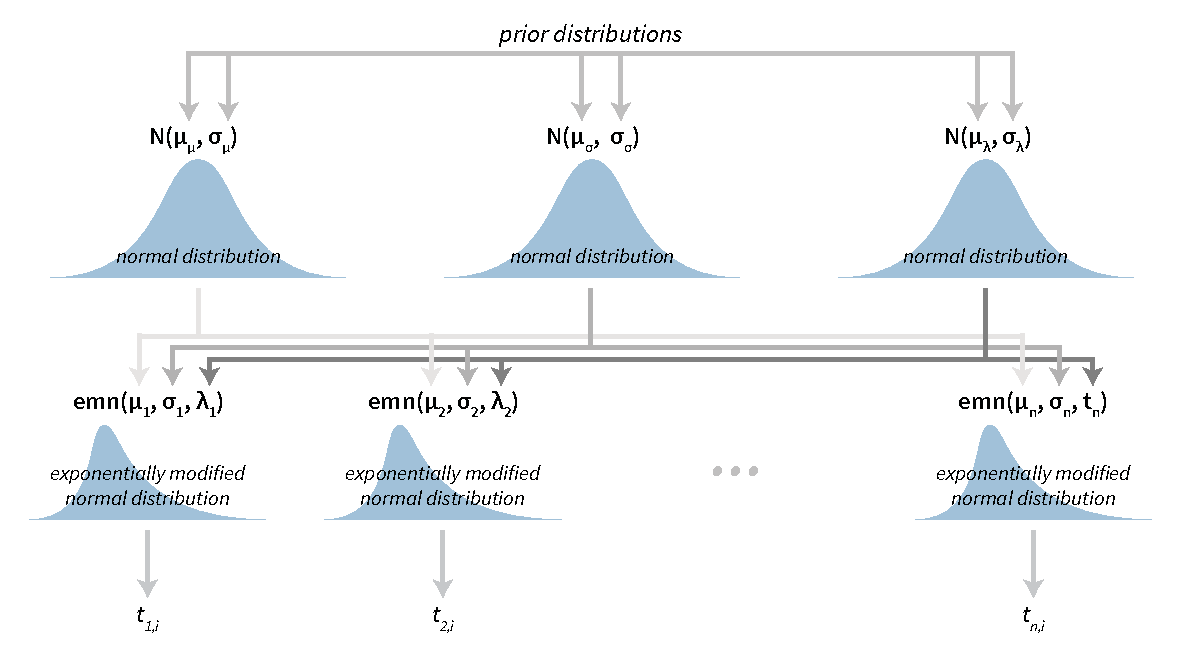
\includegraphics[width=\linewidth]{whole_page.pdf}
	\caption{\textbf{Visualization of a Bayesian hierarchical model.} This is an example of a figure that spans the whole width of the report.}
	\label{fig:whole}
\end{figure*}


\subsection*{Tables}

Use the table environment to insert tables.

\begin{table}[hbt]
	\caption{Table of grades.}
	\centering
	\begin{tabular}{l l | r}
		\toprule
		\multicolumn{2}{c}{Name} \\
		\cmidrule(r){1-2}
		First name & Last Name & Grade \\
		\midrule
		John & Doe & $7.5$ \\
		Jane & Doe & $10$ \\
		Mike & Smith & $8$ \\
		\bottomrule
	\end{tabular}
	\label{tab:label}
\end{table}


\subsection*{Code examples}

You can also insert short code examples. You can specify them manually, or insert a whole file with code. Please avoid inserting long code snippets, advisors will have access to your repositories and can take a look at your code there. If necessary, you can use this technique to insert code (or pseudo code) of short algorithms that are crucial for the understanding of the manuscript.

\lstset{language=Python}
\lstset{caption={Insert code directly from a file.}}
\lstset{label={lst:code_file}}
\lstinputlisting[language=Python]{code/example.py}

\lstset{language=R}
\lstset{caption={Write the code you want to insert.}}
\lstset{label={lst:code_direct}}
\begin{lstlisting}
import(dplyr)
import(ggplot)

ggplot(diamonds,
	   aes(x=carat, y=price, color=cut)) +
  geom_point() +
  geom_smooth()
\end{lstlisting}

%------------------------------------------------

\section*{Results}

Use the results section to present the final results of your work. Present the results in a objective and scientific fashion. Use visualisations to convey your results in a clear and efficient manner. When comparing results between various techniques use appropriate statistical methodology.

\subsection*{More random text}

This text is inserted only to make this template look more like a proper report. Lorem ipsum dolor sit amet, consectetur adipiscing elit. Etiam blandit dictum facilisis. Lorem ipsum dolor sit amet, consectetur adipiscing elit. Interdum et malesuada fames ac ante ipsum primis in faucibus. Etiam convallis tellus velit, quis ornare ipsum aliquam id. Maecenas tempus mauris sit amet libero elementum eleifend. Nulla nunc orci, consectetur non consequat ac, consequat non nisl. Aenean vitae dui nec ex fringilla malesuada. Proin elit libero, faucibus eget neque quis, condimentum laoreet urna. Etiam at nunc quis felis pulvinar dignissim. Phasellus turpis turpis, vestibulum eget imperdiet in, molestie eget neque. Curabitur quis ante sed nunc varius dictum non quis nisl. Donec nec lobortis velit. Ut cursus, libero efficitur dictum imperdiet, odio mi fermentum dui, id vulputate metus velit sit amet risus. Nulla vel volutpat elit. Mauris ex erat, pulvinar ac accumsan sit amet, ultrices sit amet turpis.

Phasellus in ligula nunc. Vivamus sem lorem, malesuada sed pretium quis, varius convallis lectus. Quisque in risus nec lectus lobortis gravida non a sem. Quisque et vestibulum sem, vel mollis dolor. Nullam ante ex, scelerisque ac efficitur vel, rhoncus quis lectus. Pellentesque scelerisque efficitur purus in faucibus. Maecenas vestibulum vulputate nisl sed vestibulum. Nullam varius turpis in hendrerit posuere.

Nulla rhoncus tortor eget ipsum commodo lacinia sit amet eu urna. Cras maximus leo mauris, ac congue eros sollicitudin ac. Integer vel erat varius, scelerisque orci eu, tristique purus. Proin id leo quis ante pharetra suscipit et non magna. Morbi in volutpat erat. Vivamus sit amet libero eu lacus pulvinar pharetra sed at felis. Vivamus non nibh a orci viverra rhoncus sit amet ullamcorper sem. Ut nec tempor dui. Aliquam convallis vitae nisi ac volutpat. Nam accumsan, erat eget faucibus commodo, ligula dui cursus nisi, at laoreet odio augue id eros. Curabitur quis tellus eget nunc ornare auctor.


%------------------------------------------------

\section*{Discussion}

Use the Discussion section to objectively evaluate your work, do not just put praise on everything you did, be critical and exposes flaws and weaknesses of your solution. You can also explain what you would do differently if you would be able to start again and what upgrades could be done on the project in the future.


%------------------------------------------------

\section*{Acknowledgments}

Here you can thank other persons (advisors, colleagues ...) that contributed to the successful completion of your project.


%----------------------------------------------------------------------------------------
%	REFERENCE LIST
%----------------------------------------------------------------------------------------
\bibliographystyle{unsrt}
\bibliography{report}


\end{document}